% Chapter 5: Conclusion

\chapter{Conclusion}
\label{sec:conclusion}

Plasma irregularities in the \(F\)-region ionosphere have been observed for decades.  However, despite extensive data sets collected over these years, surprisingly little is known about these irregularities, especially at small scales.  This is in part due to the complex and turbulent nature of the ionosphere, particularly in the polar regions, but also due to some of the inherent limitations in traditional observation techniques which can make it very challenging to identify exactly what processes are operational.  In Section \ref{sec:summary}, we summarize the results that have previously been discussed in Chapters \ref{sec:paper1}--\ref{sec:paper3}, and consider what overarching conclusions can be derived from them.  In the following Section \ref{sec:futurework}, we also provide recommendations for future research which will help answer some of the still outstanding questions and further our understanding of small-scale polar \(F\)-region plasma irregularities.

\section{Summary of Results and Conclusions}
\label{sec:summary}

Figure \ref{fig:conclusion} summarizes the major results from this body of work.  From the experimental results presented in Chapter \ref{sec:paper1}, radar backscatter from ionospheric irregularities is most likely to be observed at particular slant ranges in the radar FoV, Figure \ref{fig:conclusion}.  The location of this window of high echo occurrence varies diurnally and seasonally, primarily due to the changing background plasma density in the ionosphere.  The background density controls how far a radar beam must travel to be perpendicular to the magnetic field and to eventually be scattered back from FAIs.  This can create an appearance that small-scale plasma irregularities are more common in certain physical locations while in reality, they may exist over a much wider area but it is easier to observe them in particular locations. 

It was also demonstraighted in Chapter \ref{sec:paper1} that, in the polar caps, backscatter is often observed at nighttime even when background plasma density is low and propagation conditions are traditionally thought to be too poor for FAIs to be observed with a HF radar.  This implies an additional source of nighttime plasma density that is not easily accounted for by models.  Frequent polar patches that propagate from the dayside to the nightside could be the source of this additional density, Figure \ref{fig:conclusion}.  The requirements for confirming this hypothesis will be detailed further in Section \ref{sec:fw_patches}.

\begin{figure}
  \includegraphics[width=\textwidth]{conclusion.pdf}
  \caption[Irregularity production factors]{Summary of the main conclusions in this thesis.  The radar of interest (MCM) is highlighted in pink.  Polar patches (orange) drift antisunwards across the polar cap following the background plasma convection (red contours).  Nighttime irregularity observation is enhanced for a positive IMF \(B_y\) component.  Production is maximized near the terminator.  Small-scale irregularity production surrounding a large-scale structure is found to exhibit both asymmetry and anisotropy.  Radars are most likely to observe this asymmetry if the patch is elongated along the radar boresight.  Backscatter is most likely to be observed in a particular window of slant ranges within the radar FoV.}
  \label{fig:conclusion}
\end{figure}

One other result presented in Chapter \ref{sec:paper1} was that nighttime occurrence of FAIs was also higher for time intervals with a positive IMF \(B_y\) component, Figure \ref{fig:conclusion}.  This could be due to the control that the \(B_y\) component exerts over ionospheric convection patterns, as explained below.  In a classical two-cell convection pattern with predominantly negative IMF \(B_z\), the plasma flows antisunward from dayside to nightside across the terminator.  In this configuration, the plasma flow, \(\vec{V}_E\), and the density gradient, \(\vec{G}\), are antiparallel, the least favorable orientation for GDI growth.  However, with a significant IMF \(B_y\) component, the orientation of the convection cells rotates such that plasma no longer convects directly antisunward, creating a situation where GDI is more favorable and plasma structures can develop more readily.  Additionally, a significant IMF \(B_y\) component can contribute to the formation of polar patches by creating convection perturbations that separate high density patches from the daytime reservoir, as described in Section \ref{sec:lit_patches}.  In this way, the IMF \(B_y\) component may be indirectly responsible for the increased observation of backscatter.  If patch occurrence increases, it can contribute to the nighttime background density, as described above, which can improve propagation conditions so that FAIs can be observed by 
HF radars.

In addition to simply providing additional background density so nighttime propagation conditions are sufficient for the radar to observe FAIs, polar patches can contribute to plasma irregularity formation directly by providing background density gradients on which GDI can operate.  This raises the important question of exactly how and where plasma structures form around polar patches.  Observations have long suggested there is asymmetry in plasma structuring surrounding polar patches \citep{Weber1984,Milan2002b,Koustov2012}, but the results presented in Chapters \ref{sec:paper2} and \ref{sec:paper3} suggest that production may also be anisotropic, Figure \ref{fig:conclusion}.  

%An important conclusion that can be derived from this work is, therefore, that asymmetry and anisotropy are independent such that the plasma structures can exhibit either of them independently or both or neither.

%The other group of results presented in Chapters \ref{sec:paper2} and \ref{sec:paper3} is related to the fact that the plasma drift and wavevector directions influence the asymmetry that is observed near polar patches.  

In Chapter \ref{sec:paper2}, it was demonstrated from the modeling point of view that the direction that the patch is drifting relative to its elongation direction impacts the orientations of \(\vec{G}\) and \(\vec{V}_E\) and controls the GDI growth rate.  This also creates asymmetry between the leading and trailing edges of the patch because when the gradient direction switches, the irregularity growth rate changes from positive to negative (or vise versa) and irregularity damping occurs instead of growth.  

Additionally, linear theory predicts that the irregularity growth rate is depends on the wavevector direction, \(\uvec{k}\), so instability growth may anisotropic and the orientation of the patch and convection velocity relative to the radar, not just relative to each other, can also impact the observed irregularities.  In Chapter \ref{sec:paper2}, it was demonstrated that, in the \(F\) region, the GDI growth rate is highest for wavevectors perpendicular to the gradient, \(\vec{G}\).  Although plasma waves can occur in all directions, a SuperDARN radar will only observe waves whose wavevectors are antiparallel to a radar beam, due to the Bragg scatter condition.  Because of this, irregularity growth rate as well as structure asymmetry are most likely to be maximized if the radar's boresight is parallel to the structure's elongation, Figure \ref{fig:conclusion}.  This is further confirmed by the results of Chapter \ref{sec:paper3}, where the GDI growth rate was calculated from measurements of the density gradient, convection electric field, and wavevector direction.  When the relative orientations of all three quantities results in a positive GDI growth rate, the occurrence of plasma irregularities is greater.  An important conclusion that can be derived from this work is, therefore, that while asymmetry and anisotropy are independent processes, the small-scale plasma structuring surrounding polar patches seems to exhibit both.

In addition to large-scale density structures such as polar patches, the solar terminator can also serve as a source of density gradients required for the gradient-drift instability to operate.  In Chapter \ref{sec:paper1}, experimental evidence was presented that plasma irregularities are observed most often close to the terminator.  In addition, if a SuperDARN radar itself is positioned close to the terminator, it is observing the density gradient along its boresight, Figure \ref{fig:conclusion}.  As was demonstrated in Chapter \ref{sec:paper2} and discussed above, if small-scale irregularity growth is directionally dependent, this is also the optimal orientation from which to observe the plasma structures, leading to increased echo occurrence.  Thus modeling presented in Chapter \ref{sec:paper2} provide an alternative interpretation of earlier experimental results presented in Chapter \ref{sec:paper1}.

%The production and characteristics of small-scale plasma irregularities and the factors that control them are complex.  Radar studies must differentiate between production and propagation factors, determining if in fact irregularity production is more favorable or if background conditions just make observations of irregularities more likely.  This thesis helps advance our understanding by identifying a number of situations where small-scale irregularities are observed and establishing plausible reasons why either production is favorable according to plasma theory or radar observation is likely.

\section{Recommendations for Future Research on \(F\) Region Plasma Irregularities}
\label{sec:futurework}

Although much progress has been made in understanding small-scale plasma structuring using HF radar observations, many of the results presented in this thesis give rise to further questions that must be addressed.  In this section, four groups of possible follow-up studies are discussed.  These incude 
\begin{enumerate*}[label={(\arabic*)}] 
	\item statistical studies of polar patches using SuperDARN, 
	\item modeling of the gradient-drift instability growth rates at decameter scales, 
	\item multi-radar observations of irregularity characteristics near large-scale density gradients, and 
	\item investigation of the role of fractional perturbation density in controlling the irregularity power and occurrence.
\end{enumerate*}

\subsection{Polar Patches in SuperDARN Observations}
\label{sec:fw_patches}
In Chapter \ref{sec:paper1}, it was found that the occurrence of radar backscatter during nighttime in the polar cap is much higher than expected, particularly given that raytracing simulations predict that the orthogonality condition is rarely met and therefore there should be little to no backscatter, Figure \ref{fig:month_avg_occ}.  A hypothesis proposed in Chapter \ref{sec:paper1} was that polar patches, which are not typically well represented by ionospheric density models, occur frequently in the nighttime \(F\) region and, on average, enhance the background plasma density enough that propagation conditions are sufficient for HF radar backscatter to regularly be observed.  Experimental surveys of polar patches have shown low occurrence at nighttimes, however the occurrence of patches and their intensity increase at equinox \citep{Rodger1996}, which is where frequent nighttime backscatter is predominantly observed according to our observations, Chapter \ref{sec:paper1}.  The expected signature in the radar data from this kind of scenario would be a night with a series of isolated ``patches'' of backscatter.  An example of such an event was presented, Figure \ref{fig:patchy_example}, but it is unknown how often events like this occur.  Additionally, the intensity and size of a patch necessary to cause the radar beam to refract sufficiently must be established, possibly through further use of raytracing simulations with customizable density profiles.

\subsection{GDI Theory and Modeling at Decameter Scales}
\label{sec:fw_gdi}
One of the major drawbacks to linear GDI theory is that it inherently assumes long wavelengths, which means that in the \(F\) region, it may not be directly applicable to decameter-scale irregularities measured by HF radars.  Generally, it is assumed that some form of turbulent cascade connects plasma structures of different scale sizes in the ionosphere such that predictions made at large scales can still be applied to decameter-scale observations \citep{Tsunoda1988}.  This helps explain some of the observations of asymmetry around polar patches, which is predicted at large scales but often observed at decameter scales with radars \citep[e.g.][]{Milan2002b,Koustov2012}.  This asymmetry was also confirmed from the results presented in Chapter \ref{sec:paper2}.  However, these results also predicted anisotropy in the growth rate, which is more challenging to confirm from small-scale irregularity observations, although some evidence of such has been provided in Chapter \ref{sec:paper3}.  It may be possible to further the theoretical understanding of GDI at small scales by developing a 3D picture using kinetic theory.  \citet{Basu1995} developed such a formulation for a specific vector geometry throughout all altitudes within the ionosphere, but expanding this to general vector directions would not be trivial.  However, modeling irregularity growth with such a formulation may be necessary in order to further our understanding of how plasma structures develop at such small scales.

\subsection{Multi-Radar Observations of Irregularities and Density Gradients}
\label{sec:fw_multiradar}
The results presented in Chapter \ref{sec:paper3} could also be improved with a more extensive data set.  A single event chosen for analysis in that study was selected on the basis of good data coverage from both RISR-N and RKN and a strong density gradient being apparent in the overlapping FoV.  A recent deployment of the southern-looking face of the Resolute Bay Incoherent Scatter Radar, also known as RISR-Canada or RISR-C, Figure \ref{fig:isrmap}, created new opportunities in this area.  The observations between both radars can be coordinated and they can act as a single instrument with a FoV twice as large.  This allows a polar patch to be tracked over a longer distance and more individual data points to be captured.  Additionally, specific modes can be utilized that give a much finer grid of RISR beams, allowing measurements to be made closer together and smaller scale gradients to be evaluated.  The downside to these modes is that it takes longer for each set of measurements to be made so that the temporal resolution becomes poorer.  However, the required integration time for an ISR decreases if the background ionospheric density is higher, so the temporal resolution can improve for measurements taken during summer or daytime.  Another advantage to the RISR-N/RISR-C setup is that the SuperDARN radars at Clyde River (CLY) and Inuvik (INV) (Figure \ref{fig:superdarnmap}) cover at least part of the RISR-N/RISR-C FoV and observe it from different directions.  This presents an unique opportunity to further investigate the directional dependence of small-scale irregularities by observing the differences in backscatter observed from the same scattering volume at different directions.  Although straight-forward in theory, this experiment would most likely prove nontrivial in practice for the following reasons.  Backscatter tends to be limited spatially to the statistical high occurrence band shown in Figure \ref{fig:month_avg_occ}, and at least with INV, this band probably occurs at closer ranges than needed, so coincident backscatter is probably rare.  The probability of backscatter being observed is better when the background density is within the range where propagation conditions are most favorable, i.e. when the ionosphere is sunlit for this case.  Additionally, it is advantageous to choose a time when the occurrence of backscatter is statistically high.  Based on results from Chapter \ref{sec:paper1}, the best time for such an experiment would therefore be daytime near equinox.

\subsection{Irregularity Characteristics and Fractional Perturbation Density}
\label{sec:fw_fracdens}
In Chapter \ref{sec:paper3}, both the occurrence and power of radar backscatter are used as proxies to indicate the ``amount'' of irregularities that exist in the ionosphere.  However, the trends from these quantities are rarely in good agreement, giving rise to the question what, if anything, does each of them indicate about the plasma structuring in the ionosphere.  The factors that control each need to be isolated, but this is nontrivial.  Echo occurrence trends generally agree with the linear GDI theory predictions, but this is generally not the case for echo power.  Irregularities may develop as predicted by linear GDI theory when their amplitudes are small but other processes may impact larger density perturbations, such as shear-driven instabilities \citep{Gondarenko2006} or multistep processes \citep{Carlson2012}.  \(B_y\) the radar equation, the power returned should be proportional to the product of the background density and fractional density, squared, Equation \ref{eqn:fractional_density}.  However, there is no general consensus on what controls the fractional density in the \(F\) region, although it has been suggested that it is either constant or a function of convection speed, \(V_E\) \citep{Kustov1988,Haldoupis1990,Makarevich2014b}.  In Chapter \ref{sec:paper3}, we additionally propose that it may be a function of the instability growth rate, \(\gamma\).  Because ground-based radars are so often used to investigate ionospheric irregularities, this is an important issue to resolve to develop an accurate picture of how radar observations relate to plasma irregularities.

Our understanding of ionospheric plasma irregularities is in no way complete.  The issues outlined in this section are a small subset of questions to be addressed by future research.  Ground-based radar systems such as those employed extensively in this thesis will undoubtedly play an important role in this work.  The widespread nature of the SuperDARN network makes it ideal for statistical studies of small-scale irregularities and mapping large-scale convection.  Although scarcer, ISRs can provide a great wealth of data products, often in quite high resolution.  Other instruments, e.g. satellites, ASIs, and ASIPs, can further supplement future studies of ionospheric irregularities.  Equally important are models and theoretical studies of GDI as well as other instability mechanisms that provide insight as to how instabilities develop and explain observed trends.  Ionospheric irregularities are part of a complex system and there are still many open questions about them, but the work presented here has advanced our understanding of their characteristics, development, and where and when we can expect to observe them.

\bibliographystyle{uafthesis}
\bibliography{references}
